\documentclass{standalone}
\usepackage{amsmath}
\usepackage{tikz}
\def\D{\mathrm{d}}
\begin{document}

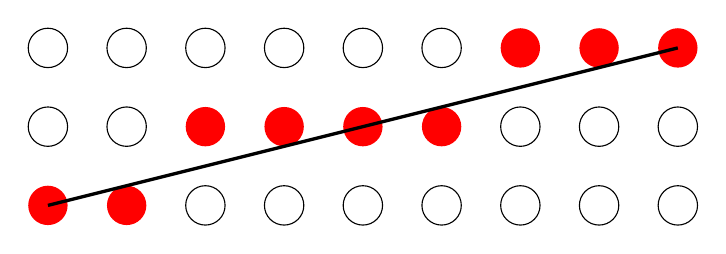
\begin{tikzpicture}

\fill[red] (0,0) circle (0.25);
\fill[red] (1,0) circle (0.25);
\draw (2,0) circle (0.25);
\draw (3,0) circle (0.25);
\draw (4,0) circle (0.25);
\draw (5,0) circle (0.25);
\draw (6,0) circle (0.25);
\draw (7,0) circle (0.25);
\draw (8,0) circle (0.25);

\draw (0,1) circle (0.25);
\draw (1,1) circle (0.25);
\fill[red] (2,1) circle (0.25);
\fill[red] (3,1) circle (0.25);
\fill[red] (4,1) circle (0.25);
\fill[red] (5,1) circle (0.25);
\draw (6,1) circle (0.25);
\draw (7,1) circle (0.25);
\draw (8,1) circle (0.25);

\draw (0,2) circle (0.25);
\draw (1,2) circle (0.25);
\draw (2,2) circle (0.25);
\draw (3,2) circle (0.25);
\draw (4,2) circle (0.25);
\draw (5,2) circle (0.25);
\fill[red] (6,2) circle (0.25);
\fill[red] (7,2) circle (0.25);
\fill[red] (8,2) circle (0.25);

\draw[very thick] (0,0) -- (8,2);
\end{tikzpicture}

\end{document}
